\documentclass[a4paper, oneside, fontsize=12pt]{scrartcl}
\usepackage[utf8]{inputenc}
\usepackage[T1]{fontenc}
\usepackage[ngerman]{babel}
\usepackage[all]{nowidow}
\usepackage[final]{listings}
\usepackage{tabularx}
\usepackage{caption}
\usepackage[title]{appendix}
\usepackage{mathptmx}
\usepackage{setspace}
\usepackage[backend=biber,style=numeric-comp,citestyle=verbose-note,autocite=footnote,labelnumber=true]{biblatex}
\usepackage{graphicx}
\usepackage[german]{csquotes}
\usepackage{fancyhdr}
\usepackage{geometry}
\usepackage{titlesec}
\newcommand{\sectionbreak}{\clearpage}
\geometry{top=30mm, bottom=30mm, left=30mm,right=25mm}


\fancypagestyle{sta}{%
  \fancyhf{}%clear all headers and footers fields
  \chead{\thepage} %prints the page number on the right side of the header
}

\bibliography{src.bib}

\lstset{
  basicstyle=\ttfamily,
  columns=fullflexible,
  frame=single,
  breaklines=true,
  postbreak=\mbox{$\hookrightarrow$\space},
}

\renewcommand{\baselinestretch}{1.3}

\begin{document}
\pagestyle{sta}
\pagenumbering{Roman}
\newgeometry{top=9.5cm, bottom=55mm, right=3cm, left=3cm}
\begin{titlepage} % Suppresses displaying the page number on the title page and the subsequent page counts as page 1
  \setstretch{1}
	
	\center % Centre everything on the page
	
	\textbf{\Large Buchstaben der Gesetze - Gesetze der Buchstaben}\\[0.5cm]
	\textbf{\large Zur Beziehung von Literatur und Recht}\\[0.5cm]

  \vspace{3cm}

	\textbf{\Large B a c h e l o r a r b e i t}\\[0.8cm]
	
	\textbf{an der Hochschule für Angewandte Wissenschaften Hof\\
  Fakultät Informatik\\
  Studiengang Allgemeine Informatik}\\[0.5cm]
	
  \vfill\vfill\vfill

	\begin{minipage}{0.4\textwidth}
		\begin{flushleft}
			\textbf{Vorgelegt bei\\
      Prof. Dr. XY\\
      Alfons-Goppel-Platz 1\\
      95028 Hof
      }
		\end{flushleft}
	\end{minipage}
	~
	\begin{minipage}{0.4\textwidth}
		\begin{flushright}
			\textbf{
      vorgelegt von\\
      Christopher Roßbach\\
      Mtr. Nr.: 01234567\\
      Street 42\\
      09226 City
      }
		\end{flushright}
	\end{minipage}
	
  \vfill

	
	\textbf{Hof,~\today} % Date, change the \today to a set date if you want to be precise
	
	
\end{titlepage}
\restoregeometry

\title{\mytitle}
\author{%
  \myname{} (\mymatrnr)%
}
\newpage
{
\setstretch{1}
\tableofcontents
\clearpage
% \addcontentsline{toc}{section}{\listfigurename}
\listoffigures
\setstretch{0.7}
\addtocontents{toc}{\protect\setcounter{tocdepth}{0}}
\glsenablehyper
\printnoidxglossary[style=long3col,title=Abkürzungsverzeichnis]
\addtocontents{toc}{\protect\setcounter{tocdepth}{3}}
\setstretch{1}
% \addcontentsline{toc}{section}{\lstlistlistingname}
\lstlistoflistings
\listoftables
\setcounter{table}{0}
}

\clearpage
\pagenumbering{arabic}
\section{Einleitung}
  Kurze Einleitung in das Thema

% main content of thesis here
\section{Hauptkapitel 1}
\subsection{sub 1}
\subsubsection{subsub 1}
... bla bla. Der Code in Listing~\ref{buffer-overflow.c} ergibt diese Ausgaben:
\begin{lstlisting}[caption={Schreiben Arraygrenzen hinaus, lesen bis Segmentation fault},label=buffer-overflow.term]
$ gcc -O0 -o buffer-overflow buffer-overflow.c
$ ./buffer-overflow
a
a
a
a
a
:
 
 
x
... 6122 Zeilen ausgelassen ...
g
_
c
o

Segmentation fault (core dumped)
\end{lstlisting}

\section{Hauptkapitel 2}
... Ein Bild:

\begin{figure}[h]
  \frame{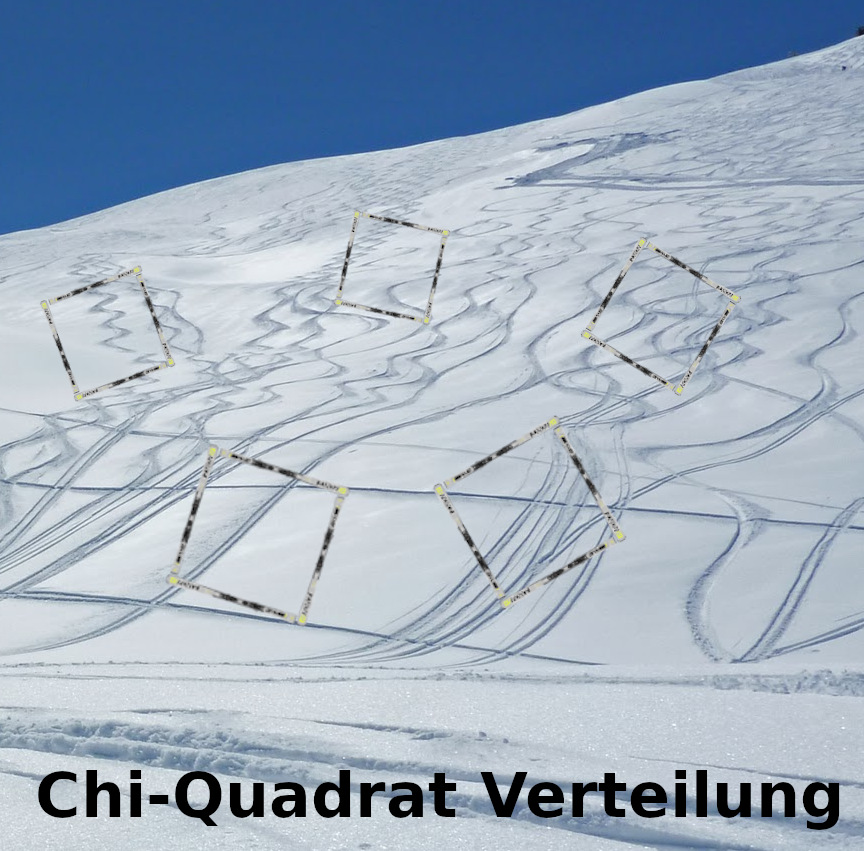
\includegraphics[width=\linewidth]{img/sample}}
  \caption{Überflüssige Bildunterschrift}\label{img-sample}
\end{figure}

Und Abkürzungen: \gls{bpel},\glspl{cli}, \glstext{aws}.

\section{Schluss}
  Einige Schlusssätze

\appendices
\clearpage
\section{Listings}
\setstretch{1}
\begin{lstlisting}[language=c,caption=\texttt{buffer-overflow.c}: C Programm Buffer Overflow, label=buffer-overflow.c]
#include <stdio.h>

int main(){
    char buff[2];

    for(int i = 0; i < 5; ++i)
        buff[i] = 'a';

    for(size_t i = 0; i < 1000000; ++i)
        printf("%c\n", buff[i]);
}
\end{lstlisting}


\clearpage
\printbibliography

\end{document}
